% !TeX root = main.tex
%  Filename   : preamble.tex
%  Description: Preamble file to :
%               a. specify related packages
%               b. set margins, commands, etc.
%\documentclass[12pt,titlepage,oneside, letterpaper]{article}
\documentclass[12pt,titlepage,oneside, letterpaper]{report}
%
%-- specify related packages
% \usepackage[utf8x]{inputenc}
\usepackage{pdfpages}
\usepackage{apacite}         %-- APA style citation  http://www.ctan.org/tex-archive/biblio/bibtex/contrib/apacite/
\usepackage{amsmath}       % American Math Society packages
\usepackage{amsfonts}
\usepackage{amssymb}
\usepackage{graphicx}      %needed for including figures in JPG or PNG format
 \usepackage{verbatim}     % tmultiple lines of comments
                               %-- example:
                               %   \begin{comment}
                               %        ...your text here...
                               %   \end{comment}  
\usepackage{color}  %-- allows use of color with text
                               %-- example:  \textcolor{red}{This is the colored text in red.}
\usepackage{url}  %-- allows use of URLs example: \url{https:\ccs1.dlsu.edu.ph}


%
%-- set margins,  you may need to edit this for your own printer
%
\topmargin 0.0in
\oddsidemargin 0.0in
\evensidemargin 0.0in

\voffset 0.0in
\hoffset 0.5625in

\textwidth 5.75in
\textheight 8.5in


\parskip 1em
\parindent 0.25in

% Bibliography style is set in main.tex.            %-- use APA citation scheme
\hyphenation{ana-lysis know-ledge}     %-- LaTeX may not hyphenate correctly some words you use in your document
                                       %-- use \hyphenation to instruct LaTeX how to do it correctly, example above
\newcommand{\degree}{^{\circ}}         %-- use \newcommand to create your own "commands"
\newcommand{\etal}{et al.}
\newcommand{\figref}[1]{Figure \ref{#1}}
\newcommand{\appref}[1]{Appendix \ref{#1}}

%\newcommand{\Section}[1]{\section{#1}\setcounter{figure}{0}\setcounter{table}{0}}

%\newcommand{\shade}{\multicolumn{1}{|>{\columncolor[gray]{0.25}}c|}{}}
%\newcommand{\tableheader}[1]{\rowcolor{black}\color{white}{#1}}
%\newcommand{\cell}[2]{\multicolumn{1}{#1}{#2}}
%\newcommand{\definition}[2]{\textbf{\textit{#1}} --- #2}
%\newcommand{\itembit}[1]{\item \textbf{\textit{#1}}}
%\newcommand{\sgdef}[2]{\parbox[t][][t]{1.75in}{\textbf{#1}} \> \parbox[t][][t]{4.0in}{#2}\\\\}

%\newenvironment{sinagglossary}{\begin{flushleft}
%\begin{tabbing}
%\hspace{1.75in}\=\\}{\end{tabbing}\end{flushleft}}

\newcommand{\thestitle}[1]{{\Large \textsc{#1}}}


%---
%  \renewcommand{\thefigure}{\thesection.\arabic{figure}}
%  \renewcommand{\thetable}{\thesection.\arabic{table}}
%  \renewcommand{\contentsname}{Table of Contents}

\graphicspath{{images/}}
\begin{document}
% !TeX root = ../main.tex
%   Filename    : title_page.tex 
\begin{titlepage}
\centering

%-- **EDIT** the following line to indicate your thesis title
\thestitle{Thesis Title}

\vspace{1.75cm}
A Special Problem\\
Presented to\\
the Faculty of the Division of Physical Sciences and Mathematics\\
College of Arts and Sciences\\
University of the Philippines Visayas\\
Miag-ao, Iloilo

\vspace{1.75cm}
In Partial Fulfillment\\
of the Requirements for the Degree of\\
Bachelor of Science in Computer Science
\vspace{1.75cm}
by\\

\vspace{1cm}
% list in alphabetical order by lastnames
MAGADAN, Jasmine  \\
YAP, Mae Maricar  \\
% LASTNAME4, FirstName4  \\

\vspace{1.75cm}
Francis DIMZON, Ph.D. \\
Adviser\\
%Firstname LASTNAME \\
%Co-Adviser

\vspace{1.75cm}
\today
\end{titlepage}

% !TeX root = ../main.tex
%   Filename    : abstract.tex 
\begin{abstract}
From 150 to 200 words of short, direct and complete sentences, the abstract 
should be informative enough to serve as a substitute for reading the entire SP document 
itself.  It states the rationale and the objectives of the research.  
In the final Special Problem  document (i.e., the document you'll submit for your final defense), the  abstract should also contain a description of your research results, findings,  and contribution(s).

%  Do not put citations or quotes in the abract.

Suggested keywords based on ACM Computing Classification system can be found at \url{https://dl.acm.org/ccs/ccs_flat.cfm}

\begin{flushleft}
\begin{tabular}{lp{4.25in}}
\hspace{-0.5em}\textbf{Keywords:}\hspace{0.25em} & Keyword 1, keyword 2, keyword 3, keyword 4, etc.\\
\end{tabular}
\end{flushleft}
\end{abstract}

\pagenumbering{roman}
\setcounter{page}{2}
\tableofcontents
\clearpage
\listoffigures
\clearpage
\listoftables
\clearpage
\pagenumbering{arabic}
% !TeX root = ../../main.tex
%   Filename    : chapter_1.tex 
\chapter{Introduction}
\label{chap:chap1}
\label{sec:researchdesc}    %labels help you reference sections of your document

\section{Overview of the Current State of Technology}
\label{sec:overview}

This section gives the reader an overview of the specific technology or field in the international or
local setting. 
The information regarding the technology or field should be contemporary and not based on outdated sources. 
Discussion must not be too technical or too detailed.
   
\textcolor{red}{This section ends with a discussion on the problem/s faced by or that still exist in the specific
technology or field (e.g., limitations of existing software or algorithms). 
The problem statement would lead to the research objectives.}


It is   easy to include a figure in JPG or PNG format as shown in the  following example.  
Make sure that you explain what the figure is all about, and that you refer to your figure.  
For example, \figref{fig:disneystock} shows a graph of the performance of Disney stock from the 1980s to 2012.
  
%--- the following example shows how to include a figure in PNG format
\begin{figure}[t]                %-- use [t] to place figure at top, [b] to place at the bottom, [h] for here
   \centering                    %-- use this to center the figure
   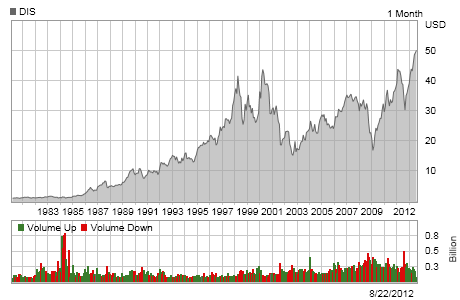
\includegraphics{DisneyChart.png}      %-- include image file named as "disneychart.png" 
   \caption{This is the figure's caption -- Disney stock chart.
   	Captions should fully describe the figure in a concise manner  such that there is not need to refer to the text when figuring out the graphic.}
    \label{fig:disneystock}
\end{figure}


Some notes on citing references.   
When using APA format, the author-date method of citation is  followed.   
This means that the author's last name and the year of publication for the source should  appear in the text, and a complete reference should appear in the reference list.

% Examples:
%     	Smith (1970) compared reaction times . . .
%     	In a recent study of reaction times (Smith, 1970), . . .   
%     	In 1970, Smith compared reaction times . . .
%	    Smith, et al., (1970) compared reaction times . . .
%     	In a recent study of reaction times (Smith, et al., 1970), . .
%     	In 1970, Smith, et al., compared reaction times . . .

Here are some examples on how to do the referencing (note author's name and years are different from commented examples).  
For APA citation details, refer to \url{http://www.ctan.org/tex-archive/biblio/bibtex/contrib/apacite/}. 

\begin{itemize}
 \item \citeA{kartch:2000:ERA} compared reaction times...
 \item In a recent study of reaction times \cite{kartch:2000:ERA}...
 \item In \citeyearNP{kartch:2000:ERA}, \citeauthor{kartch:2000:ERA} compared reaction times...
 \item \shortciteA{fedkiw:2001:VSO} compared reaction times... 
 \item In a recent study of reaction times \cite{fedkiw:2001:VSO}...
 \item In \citeyearNP{fedkiw:2001:VSO}, \shortciteauthor{fedkiw:2001:VSO}, compared reaction times...
\end{itemize}

The following are references from journal articles \cite{Park:2006:DSI, Pellacini:2005:LAH, sako:2001:SSB}.
 Here's an MS thesis document \cite{yee:2000:SSA}, and this is from PhD dissertation \cite{kartch:2000:ERA}. 
 For a book, reference is given as  \cite{parke:1996:CFA}. 
 Proceedings from a conference samples are \cite{Jobs95, fedkiw:2001:VSO, levoy:2000:TDM}.  
 The sample bibliography file named \textbf{references.bib} is from the SIGGRAPH \LaTeX{}  template.  
 You can use a text editor to view the contents of the bib file.  
 It is your task to create your own bibliography file.  
 For those who downloaded papers from ACM or IEEE sites, there is a BibTeX link that you can click; thereafter, you just simply need to copy and paste the BibTeX entry into your own bibliography file.

The following shows how to include a program source code (or algorithm).  
The verbatim environment, as the name suggests, outputs text (including white spaces) as is...

\begin{verbatim}
               #include <stdio.h>
               main()
               {
                    printf("Hello world!\n");
               }
\end{verbatim}

\section{Problem Statement}
\textcolor{red}{DO NOT FORGET to write the statement of the research problem here, i.e., before the Research Objectives.}

A problem statement is your research problem written explicitly.  
The problem statement should do four things: 
\begin{enumerate}
	\item Specify and describe the problem (with appropriate citations) 
	\item  Provide evidence of the problem’s existence  
	\item Explain the consequences of NOT solving the problem  
	\item 	Identify what is not known about the problem that should be known.
\end{enumerate}


\section{Research Objectives}
\label{sec:researchobjectives}

\subsection{General Objective}
\label{sec:generalobjective}

This subsection states the over--all goal that must be achieved to answer the problem.
Address the following: Given your research challenge or opportunity, how do you intend  to solve it? What is the output of your research?


\subsection{Specific Objectives}
\label{sec:specificobjectives}

%
%  \begin{comment} ... \end{comment} is used for multiple lines of comment
%

This subsection is an elaboration of the general objective.  
It states the specific steps that must be undertaken to accomplish the general objective.  
These objectives must be \textbf{S}pecific, \textbf{M}easurable, \textbf{A}ttainable, \textbf{R}ealistic, \textbf{T}ime-bounded.  
A specific objective start with ``to $<$verb$>$'' for example: to design/survey/review/analyze.

Studying a particular programming language or development tool (e.g., to study Windows/Object-Oriented/Graphics/C++ programming) to  accomplish the general objective is inherent in all thesis and, therefore, must not be included here.


\begin{comment}
% IPR acknowledgement: the following sentences and examples are from Ethel Ong's slides 
%     on Research Objectives
How to formulate your research objectives:
1. Identify what research steps do you need to perform to achieve your general objective.
2. Identify the questions that must be answered for you to achieve your general objective.
    Thereafter, convert these questions into action statements

Example #1:

Research Question:
  What are the general features of a web-based learning environment?

Specific Objective:
   To review existing web-based learning environment that teaches language learning for children


Example #2:

Research Question:
   How will you represent commonsense knowledge for use by computer systems?

Specific Objective:
   To identify knowledge representation approaches used by existing story generation systems

Example #3:
Research Question:
   What types of storytelling knowledge are needed to generate stories?

Specific Objective:
    To identify the different types of storytelling knowledge used in generating stories

Example #4:
Research Question:
    What machine learning approaches will you utilize?

Specific Objective:
    To determine existing machine learning algorithms [that can be used in training the computer system to detect cyberbullying cases] 

Example #5: Research Question:
    How will your research output be evaluated?

Specific Objective:
    To define evaluation metrics for validating the accuracy of the translation

\end{comment}

%
%  The following are example specific objectives; replace them with your own 
%

\begin{enumerate}
   \item To review related literature, compare and contrast existing algorithms (on what problem?);
   \item To develop a new algorithm (for what purpose?)
   \item To analyze the algorithm (based on what criteria?)
\end{enumerate}


\section{Scope and Limitations of the Research}
\label{sec:scopelimitations}

This section discusses the boundaries (with respect to the objectives) of the research and the constraints within 
which the research will be developed.

\begin{comment}

%
% IPR acknowledgement: the sentences inside this comment are from Ethel Ong's slides on Scope and Limitations of the Research
%
Generally, one paragraph should be allotted for each of your research objectives.

Each paragraph contains a brief overview of the concept/theory and the purpose of doing the associated objective.

Each paragraph also includes a description of the scope/limitation of your study.

* Please refer to the slides for examples.

\end{comment}


\section{Significance of the Research}
\label{sec:significance}

This section explains why research must be done in this area.
 It rationalizes the objective of the research with that of the stated problem. 
 Avoid including sentences such as ``This research will be beneficial to the proponent/department/college'' as this is already an inherent requirement of all BSCS majors.  Focus on the research's contribution to the Computer Science field.

The following are guide questions that may help your formulate the significance of your research. 


%
% IPR acknowledgement: the following list of items are from Ethel Ong's slides on Significance of the Research
%
\begin{itemize}
\item  What is the relevance of your work to the computer science community? 

\begin{itemize} 
\item What will be your technical contributions, in terms of algorithms, or approaches, or new domain? 
\item What is your value-added compared to existing systems? 
\end{itemize}

\item What will be your contributions to society in general? 
    \begin{itemize}
      \item Who will benefit from your system? 
      \item Who are your target users and how will this system benefit them? 
   \end{itemize}
\end{itemize}

\begin{comment}
If applicable, describe possible commercialization and/or innovation in your research.
\end{comment}



% !TeX root = ../../main.tex
\chapter{Review of Related Literature and Studies}
\label{chap:chap2}
% !TeX root = ../../main.tex
%   Filename    : chapter_2.tex 
% Chapter heading is supplied by chapter-2-main.tex.
\label{sec:relatedlit}

This chapter discusses the features, capabilities, and limitations of existing research, algorithms, or software  that are related/similar to the Special Problem.

 The reviewed works and software must be arranged either in chronological order, or by area (from general to specific).  
Observe a consistent format when presenting each of the reviewed works. 
This must be selected in consultation with the  adviser.

\textcolor{red}{DO NOT FORGET to cite your references.}


\begin{comment}
%
% IPR acknowledgement: the contents withis this comment are from Ethel Ong's slides on RRL.
%
Guide on Writing your RRL chapter
 
1. Identify the keywords with respect to your research
      One keyword = One document section
                Examples: 2.1 Story Generation Systems
			 2.2 Knowledge Representation

2.  Find references using these keywords

3.  For each of the references that you find,
        Check: Is it relevant to your research?
        Use their references to find more relevant works.

4. Identify a set of criteria for comparison.
       It will serve as a guide to help you focus on what to look for

5. Write a summary focusing on -
       What: A short description of the work
       How: A summary of the approach it utilized
       Findings: If applicable, provide the results
        Why: Relevance to your work

6. At the end of each section,  show a Table of Comparison of the related works 
   and your proposed project/system

\end{comment}

\section{Theme 1 Title}
This chapter  contains a review of research papers that:
%
% IPR acknowledgement: the following list of items are from Ethel Ong's slides RRL.
%
\begin{itemize}
\item Describes work on a research area that is similar or relevant to yours
\item Describes work on a domain that is similar or relevant to yours
\item Uses an algorithm that may be useful to your work
\item Uses a software / tool that may be useful to your work
\end{itemize}

%\section{Review of Related Software}
It also contains a review of software systems that:
%
% IPR acknowledgement: the following list of items are from Ethel Ong's slides on RRL.
%
\begin{itemize}
   \item Belongs to a research area similar to yours
   \item Addresses a need or domain similar to yours
   \item Is your predecessor
\end{itemize}

\section{Theme 2 Title}
















% new page
\clearpage 
% !TeX root = ../../main.tex
\section{Related Literature}
\label{sec:related-literature}

This section discusses concepts and technologies relevant
to the research.

\subsection{Your First Topic}

Write your discussion here.

\subsection{Your Second Topic}

Write your discussion here.


\clearpage
% !TeX root = ../../main.tex
\section{Related Studies}
\label{sec:related-studies}

This section reviews previous studies relevant
to the research.

\subsection{Your First Study}

Discuss its objectives, methods, findings, limitations,
and relevance to your research.

\subsection{Your Second Study}

Write your discussion here.


% !TeX root = ../../main.tex
%   Filename    : chapter_4.tex 
\chapter{Research Methodology}
\label{chap:chap3}
This chapter lists and discusses the specific steps and activities that will be performed  to accomplish the project. 
The discussion covers the activities from pre-proposal to Final SP Writing.

\section{Research Activities}
Research activities include inquiry, survey, research, brainstorming, canvassing, consultation, review, interview, observe, experiment, design, test, document, etc.  
Be sure that for each method, process, or algorithm used, there is a justification why that method was chosen.
The methodology also includes the following information:

\begin{itemize}
   \item who is responsible for the task
   \item the resource person to be contacted
   \item what will be done
   \item when and how long will the activity be done
   \item where will it be done
   \item why should be activity be done
\end{itemize}


\section{Calendar of Activities}

A Gantt chart showing the schedule of the activities should be included as a table. For example:

Table \ref{tab:timetableactivities} shows a Gantt chart of the activities.  Each bullet represents approximately
one week worth of activity.

%
%  the following commands will be used for filling up the bullets in the Gantt chart
%
\newcommand{\weekone}{\textbullet}
\newcommand{\weektwo}{\textbullet \textbullet}
\newcommand{\weekthree}{\textbullet \textbullet \textbullet}
\newcommand{\weekfour}{\textbullet \textbullet \textbullet \textbullet}

%
%  alternative to bullet is a star 
%
\begin{comment}
   \newcommand{\weekone}{$\star$}
   \newcommand{\weektwo}{$\star \star$}
   \newcommand{\weekthree}{$\star \star \star$}
   \newcommand{\weekfour}{$\star \star \star \star$ }
\end{comment}



\begin{table}[ht]   %t means place on top, replace with b if you want to place at the bottom
\centering
\caption{Timetable of Activities} \vspace{0.25em}
\begin{tabular}{|p{2in}|c|c|c|c|c|c|c|c|} \hline
\centering Activities (2009) & Jan   & Feb & Mar & Apr & May & Jun & Jul \\ \hline
Study on Prerequisite Knowledge      &   &  & ~~~\weektwo & \weekfour &  &  &  \\ \hline
Review of Existing Racing Strategies & ~~~\weektwo  & \weekfour & \weekfour & \weekfour &  &  &  \\ \hline
Identification of Best Features      &   &  &  & \weekfour & \weektwo~~~ &  &  \\ \hline
Development of Racing Strategies     &   &  &  & ~~~\weektwo & \weekfour & \weektwo~~~ &  \\ \hline
Simulation of Racing Strategies      &   &  &  & ~~~\weektwo & \weekfour & \weekthree~~ &  \\ \hline
Analysis and Interpretation of the Results &   &  &  &  & \weekfour & \weekfour & \weekone~~~~~ \\ \hline
Documentation & ~~~\weektwo  & \weekfour & \weekfour & \weekfour & \weekfour & \weekfour & \weektwo~~~ \\ \hline
\end{tabular}
\label{tab:timetableactivities}
\end{table}


% !TeX root = ../../main.tex
%   Filename    : chapter_4.tex 
\chapter{Preliminary Results}
This chapter  presents the preliminary results or the system prototype of your SP.  Include screenhots, tables, or graphs and provide the discussion of results.
\appendix
% !TeX root = ../main.tex
%%%%%%%%%%%%%%%%%%%%%%%%%%%%%%%%%%%%%%%%%%%%%%%%%%%%%%%%%%%%%%%%%%%%%%%%%%%%%%%%%%%%%%%%%%%%%%%%%%%%%%
%
%   Filename    : appendix_A.tex 
%
%   Description : This file is for including the Research Ethics Documents (delegated as Appendix A) 
%                 
%%%%%%%%%%%%%%%%%%%%%%%%%%%%%%%%%%%%%%%%%%%%%%%%%%%%%%%%%%%%%%%%%%%%%%%%%%%%%%%%%%%%%%%%%%%%%%%%%%%%%%

\chapter{Appendix Title}
\label{sec:appendixa}



% Save the file you want to include in PDF format.
% Uncomment the commant below specifying the correct appendix file. 
%\includepdf[pages=-, scale = 0.9, pagecommand={}, offset = -30 0]{appendixA.pdf}


% !TeX root = ../main.tex
%%%%%%%%%%%%%%%%%%%%%%%%%%%%%%%%%%%%%%%%%%%%%%%%%%%%%%%%%%%%%%%%%%%%%%%%%%%%%%%%%%%%%%%%%%%%%%%%%%%%%%
%
%   Filename    : appendix_B.tex
%
%   Description : This file will contain information about your Resource Persons
%                 
%%%%%%%%%%%%%%%%%%%%%%%%%%%%%%%%%%%%%%%%%%%%%%%%%%%%%%%%%%%%%%%%%%%%%%%%%%%%%%%%%%%%%%%%%%%%%%%%%%%%%%

\chapter{Resource Persons}
\label{sec:appendixb}

%
%  Indicate your resource persons here:
%
%	<full name and title, e.g., Dr. Juan de la Cruz>
%	<profession, e.g., faculty>
%	<department, e.g., Division of Physical Sciences and Mathematics>
%	<name of institution, e.g., University of the Philippines Visayas>
%	<e-mail address>
%
%

%
%  the following shows 3 examples, replace entries with your own
%

\newcommand{\resperson}[4]{\textbf{#1} \\ #2 \\ #3 \\ \url{#4}\vspace{0.5em}\\}

\resperson{Dr. Firstname1 Lastname1}{Adviser}{Affiliation1}{emailaddr@domain.com}
\resperson{Mr. Firstname2 Lastname2}{Role2}{Affiliation2}{emailaddr2@domain.com}
\resperson{Ms. Firstname3 Lastname3}{Role3}{Affiliation3}{emailaddr3@domain.net}

\bibliographystyle{apacite}
% Show References even before the first BibTeX build creates main.bbl.
% Once it exists, apacite supplies both the heading and the contents entry.
\IfFileExists{\jobname.bbl}{}{%
  \clearpage
  \chapter*{\bibname}
  \addcontentsline{toc}{chapter}{\bibname}
}
\bibliography{references}
\end{document}
